% =============================================================================
% Section 9. Bilateral partnership indices
% Specification: R/themes/partnership_strength/{partnership_strength_helpers,safer_friendshore,
% cm_fdi,prosperous_opportunity,stronger_development,psi_composite}.R,
% R/indices/build_partnership_strength_index.R, scripts/15_build_partner_themes.R,
% scripts/25_build_partner_indices.R, config/weights.yml (psi, partnership_*_components),
% config/partnership.yml (trade mirror, conduits, cm_fdi), config/rankability.yml.
% Numbers: paper/results/bilateral.json (final rerun of 2026-10-12); figures and tables:
% scripts/paper/fig_bilateral.R. Further detail: sections/oa_bilateral.tex (oa:bilateral).
% =============================================================================
\section{Bilateral partnership indices}\label{sec:bilateral}

The choice of partner trades the security of trusted suppliers against the efficiency cost of
narrowing the supplier set \citep{yellen2022remarks,aiyar2023geoeconomic,gopinath2025changing,
javorcik2024economic,grossman2023supply}, and sourcing is already being reallocated across partners
\citep{alfaro2023global,freund2024us}. Its unit is the pair of countries. This section builds three
bilateral pillars and a composite: the
\emph{Friendshore} index $\FS$ rates partner $j$ as a supplier of $(t,s)$ to economy $i$; the
\emph{Partnership Opportunity} index $\PO$ rates $j$ as a market for $i$'s exports; the
\emph{Development Potential} index $\DP$ rates $j$ alone as a development partner; and the
\emph{Partnership Strength Index} $\PSI$ combines them (Table~\ref{tab:bilateral_pillars}). The
network design (Section~\ref{sec:network}) uses the dyad-level $\FS$ and $\PO$ and the partner-level
$\DP$, not the $\PSI$.

\begin{table}[tbp]
\centering
\begin{threeparttable}
\caption{The bilateral pillars: units, direction, components and weights}
\label{tab:bilateral_pillars}
\footnotesize
\begin{tabularx}{\textwidth}{@{}>{\raggedright\arraybackslash}p{2.2cm}
  >{\raggedright\arraybackslash}X >{\raggedright\arraybackslash}X
  >{\raggedright\arraybackslash}X@{}}
\toprule
 & Friendshore ($\FS$) & Partnership Opportunity ($\PO$) & Development Potential ($\DP$)\\
\midrule
Unit & dyad $\dyad$ & dyad $\dyad$ & partner $(j,t,s)$\\
Reporter $i$ & importer, sourcing $(t,s)$ & exporter of $(t,s)$ & none\\
Partner $j$ & candidate supplier & candidate export market & non-high-income economy\\
Components (weight) &
  $\tau^{M}_{ijts}$ imports from $j$ (2); $\nu_{its}$ reporter need (2); $e_{jts}$ partner $\EO$
  rank (2); $o_{ijts}$ outward investment in $j$ (2); $A_{ij}$ UNGA alignment (2); $1-\chi_{jt}$
  Chinese-parent exposure (1; four Midstream cells); reporter $\EO$ rank (0) &
  $\tau^{X}_{ijts}$ exports to $j$ (3); $\varepsilon_{its}$ reporter $\EO$ rank (3);
  $\eta_{jts}$ partner $\ES$ need (1) &
  eight partner components, weights $1,1,1,1,1.5,1.5,2,1$ (Table~\ref{tab:dp_components})\\
Climate penalty & $0.10\,(1-g_t)(\mathrm{CPI}_i+\mathrm{CPI}_j)$ & $0.05\,(1-g_t)\,\mathrm{CPI}_j$
  & none\\
Final transform & ${\Scurve}[\cdot]_{ts}$ over dyads, after flooring at 0 & ${\Scurve}[\cdot]_{ts}$
  over dyads, after flooring at 0 & ${\Scurve}[\cdot]_{ts}$ over partners\\
Summary to $\PSI$ & best five $(t,s)$ per dyad; mean over the core reporters & best five $(t,s)$
  per dyad; mean over the core reporters & best five $(t,s)$ per partner\\
$\PSI$ weight & $0.4$ & $0.4$ & $0.2$\\
\bottomrule
\end{tabularx}
\begin{tablenotes}[flushleft]\footnotesize
\item \textit{Notes:} Weights from \texttt{config/weights.yml}; within each pillar they are
renormalized over the components observed (equation~\eqref{eq:bilateral_acmean}). The $\FS$ penalty
coefficient (0.10 per side) is fixed in code, the $\PO$ coefficient configured. $g_t$ is the
technology emission weight of equation~\eqref{eq:ghg_index}, $\mathrm{CPI}$ the Climate Action
Tracker rating. In Batteries, Electric Vehicles, Solar and Wind Midstream $o_{ijts}$ is the CM-FDI
project tie and $\chi_{jt}$ is defined; elsewhere $o_{ij}$ is the IMF position and $\chi$ is absent.
\end{tablenotes}
\end{threeparttable}
\end{table}

% -----------------------------------------------------------------------------
\subsection{Dyads, trade and shared building blocks}\label{subsec:bilateral_dyads}

A dyad $\dyad$ pairs reporter $i$ and partner $j\neq i$, among 219 economies, in a headline
technology $t$ and stage $s$. In $\FS_{ijts}$ the reporter is the importer and $j$ the candidate
supplier; in $\PO_{ijts}$ the reporter is the exporter and $j$ the candidate market. Both rate $j$
from $i$'s side, so a supply edge from producer $p$ to consumer $c$ is read as $\FS_{cpts}$ and
$\PO_{pcts}$ (Section~\ref{sec:network}). ${\Scurve}[x]_{g}$ is the S-curve of
Section~\ref{sec:normalization} within each cell of grouping $g$ ($ts$: all dyads of a cell; $its$:
reporter $i$'s partners in the cell; $i$: all units of reporter $i$). Missing components are dropped
and the weights renormalized,
\begin{equation}\label{eq:bilateral_acmean}
  \mathcal{A}_{\bm w}(x_1,\dots,x_C)=\frac{\sum_{c} w_c\,x_c\,\1\{x_c\ \text{observed}\}}
  {\sum_{c} w_c\,\1\{x_c\ \text{observed}\}},
\end{equation}
so a missing component is never scored as zero.

\paragraph{Bilateral trade.}\label{subsec:bilateral_blocks} Trade comes from the all-reporter
Comtrade dyads for 2020 and 2024 \citep{uncomtrade}: the importer's own declaration where it reports
the cell, otherwise the exporter's mirror declaration times the CIF/FOB factor 1.06; a reporter that
declares no trade with a partner records a zero, and non-reporting economies enter only through
their partners' declarations. With $H_{ts}$ the HS6 basket of the cell (Section~\ref{sec:data}),
the cell flow is
\begin{equation}\label{eq:bilateral_trade_value}
  M^{y}_{ijts}=\sum_{h\in H_{ts}} m^{y}_{ijh},
\end{equation}
a product in several baskets counting in each. Among dyads that trade, the 2024 level $L$ and the
growth since 2020 $G$ are ranked within the cell and combined 2:1, then re-ranked among the
reporter's own suppliers,
\begin{equation}\label{eq:bilateral_trade_index}
  \tilde\tau^{M}_{ijts}=\mathcal{A}_{(2,1)}\bigl({\Scurve}[L]_{ts},\,{\Scurve}[G]_{ts}\bigr),
  \qquad
  \tau^{M}_{ijts}={\Scurve}\bigl[\tilde\tau^{M}\bigr]_{its},
\end{equation}
so that $\tau^{M}_{ijts}$ measures $j$'s place among $i$'s sources. Recorded zeros form one tie block
below every trading partner; a dyad with no observed 2024 flow takes the cell mean; the 15 cells
without a basket carry no trade information. The export component $\tau^{X}_{ijts}$ is built the
same way from $i$'s exports.

\paragraph{Climate penalty.} Each economy carries a Climate Action Tracker rating $\mathrm{CPI}_i$
\citep{cat2026ratings} (0.25 to 1; EU members take the EU's, unrated economies the median, 0.75).
The penalty is proportional to $(1-g_t)\,\mathrm{CPI}$, with $g_t$ the technology weight of
equation~\eqref{eq:ghg_index}. Because $g_t$ is constant within a cell, it re-orders dyads within
carbon-intensive technologies by the parties' climate ambition \citep{clausing2023carbon} rather than
lowering those technologies against clean ones.

% -----------------------------------------------------------------------------
\subsection{The Friendshore index}\label{subsec:friendshore}

Friendshore asks how good a supplier $j$ is for $i$ in $(t,s)$. Besides the import component it
has the reporter's need, ranked among its own cells, and the partner's capability, ranked across
countries,
\begin{equation}\label{eq:fs_need}
  \nu_{its}=1-{\Scurve}[\ES]_{i}(i,t,s),\qquad e_{jts}={\Scurve}[\EO]_{ts}(j,t,s),
\end{equation}
so that $\nu$ identifies which technologies $i$ should friendshore, not which countries most need
to. The dyadic alignment $A_{ij}$ of equation~\eqref{eq:coalition_dyadic} enters as it is, without
ranking.

\paragraph{Outward investment.} An outward position reveals an ownership or financing link that gives
the investor a stake in the partner's capacity. Outside four cells, $o_{ij}$ uses the reporter's
outward direct-investment debt positions in the IMF Direct Investment Positions \citep{imf2026dip},
averaged over 2020--2024 ($\bar D_{ij}$); positions involving 16 conduit financial centres,
dominated by pass-through capital \citep{damgaard2024real}, are unobserved on both sides. With $Y$
the 2023 GDP,
\begin{equation}\label{eq:outbound}
  \tilde o_{ij}=
  \begin{cases}
    \mathcal{A}_{(1,1,1)}\bigl({\Scurve}[\bar D],\ {\Scurve}[\bar D/Y_j],\ {\Scurve}[(\bar D/Y_i)/Y_j]\bigr)
      & \text{if } \bar D_{ij}>0,\\[2pt]
    0 & \text{if } \bar D_{ij}\le 0,
  \end{cases}
  \qquad
  o_{ij}={\Scurve}[\tilde o]_{i}.
\end{equation}
An absent record is missing, not zero. In Batteries, Electric Vehicles, Solar and Wind Midstream the
tie $o_{ijts}$ comes instead from the CM-FDI database of cross-border clean-technology manufacturing
projects \citep{bandara2026cmfdi}: the projects of parents headquartered in $i$ located in $j$,
ranked on attributed counts and disclosed capital within the cell and then within the reporter.

\paragraph{Chinese-parent exposure.} For supplier $j$ and technology $t$ in the same four cells,
$\chi_{jt}$ is the share of $j$'s foreign-invested manufacturing owned by parents headquartered in
China, Hong Kong or Macao: capital-weighted where capital is disclosed and by count otherwise, half
of a joint venture attributed to the listed parent, defined only where $j$ hosts at least two
projects, and set to one for China, Hong Kong and Macao. It enters as $1-\chi_{jt}$, so a supplier
whose foreign-invested capacity belongs to Chinese parents scores lower.

\paragraph{Composite and index.} With the reporter's own $\EO$ rank carried at weight zero,
\begin{equation}\label{eq:fs_raw}
  \tilde F_{ijts}=\mathcal{A}_{\bm w^{\FS}}\bigl(\tau^{M}_{ijts},\,\nu_{its},\,e_{jts},\,o_{ijts},\,
  A_{ij},\,1-\chi_{jt}\bigr),\qquad \bm w^{\FS}=(2,2,2,2,2,1),
\end{equation}
\begin{equation}\label{eq:fs_penalty}
  \pi^{\FS}_{ijt}=0.10\,(1-g_t)\,(\mathrm{CPI}_i+\mathrm{CPI}_j),
\end{equation}
\begin{equation}\label{eq:fs_index}
  \FS_{ijts}={\Scurve}\bigl[\max\bigl(0,\ \tilde F-\pi^{\FS}\bigr)\bigr]_{ts}.
\end{equation}
The index rewards a match between the reporter's weaknesses and the partner's strengths, backed by
revealed ties and political alignment.

% -----------------------------------------------------------------------------
\subsection{The Partnership Opportunity index}\label{subsec:partnership_opportunity}

A market is worth more to an exporter when the exporter is competitive in the technology, already
sells there, and the market's insecurity signals demand for new supply. With the reporter's and the
market's cross-country ranks,
\begin{equation}\label{eq:po_components}
  \varepsilon_{its}={\Scurve}\bigl[{\Scurve}[\EO]_{ts}(i,t,s)\bigr]_{ts},\qquad
  \eta_{jts}={\Scurve}\bigl[1-{\Scurve}[\ES]_{ts}(j,t,s)\bigr]_{ts},
\end{equation}
\begin{equation}\label{eq:po_index}
  \tilde P_{ijts}=\mathcal{A}_{(3,3,1)}\bigl(\tau^{X}_{ijts},\,\varepsilon_{its},\,\eta_{jts}\bigr),
  \qquad
  \pi^{\PO}_{jt}=0.05\,(1-g_t)\,\mathrm{CPI}_j,
  \qquad
  \PO_{ijts}={\Scurve}\bigl[\max\bigl(0,\ \tilde P-\pi^{\PO}\bigr)\bigr]_{ts}.
\end{equation}
Unlike the Friendshore need term, $\eta_{jts}$ compares the market's insecurity with that of other
markets. The penalty falls on the market's climate policy only.

% -----------------------------------------------------------------------------
\subsection{The Development Potential index}\label{subsec:development_potential}

Development Potential describes partner $j$ alone: its enabling environment, energy-security need,
economic opportunity, the official development assistance it receives in each stage, and its energy
use (Table~\ref{tab:dp_components}). It is defined for the 132 partners that the World Bank does not
classify as high income,
\begin{equation}\label{eq:dp_index}
  \widetilde D_{jts}=\mathcal{A}_{\bm w^{\DP}}\bigl(d^{(1)}_{jts},\dots,d^{(8)}_{jts}\bigr),\qquad
  \bm w^{\DP}=(1,1,1,1,1.5,1.5,2,1),\qquad
  \DP_{jts}={\Scurve}\bigl[\widetilde D\bigr]_{ts},
\end{equation}
ranked across eligible partners within the cell. Only need, opportunity and stage aid vary across a
partner's cells, so they decide which cells its best-five summary selects. Online
Appendix~\ref{oa:bilateral} gives the 40-series WDI basket, the aid measure and the orientation
choices.

\begin{table}[tbp]
\centering
\begin{threeparttable}
\caption{Components of the Development Potential index}
\label{tab:dp_components}
\footnotesize
\begin{tabularx}{\textwidth}{@{}l l >{\raggedright\arraybackslash}X c@{}}
\toprule
Component & Varies by & Construction & Weight\\
\midrule
$d^{(1)}$ development index & $j$ & S-curve across economies of the mean of the observed
  S-curved WDI series of a 40-series basket (2022--2024 averages; 13 inverted) & 1\\
$d^{(2)}$ business environment & $j$ & S-curve of the Doing Business score (2019, last release) & 1\\
$d^{(3)}$ investment environment & $j$ & S-curve of $(d^{(1)}+d^{(2)})/2$ & 1\\
$d^{(4)}$ energy-security need & $j,t,s$ & $1-\ES_{jts}$ & 1\\
$d^{(5)}$ economic opportunity & $j,t,s$ & $\EO_{jts}$ & 1.5\\
$d^{(6)}$ stage aid & $j,s$ & S-curve of ODA disbursements to the stage's sector (OECD CRS) & 1.5\\
$d^{(7)}$ stage aid intensity & $j,s$ & the same per unit of 2023 GDP & 2\\
$d^{(8)}$ energy use & $j$ & S-curve of energy use per capita & 1\\
\bottomrule
\end{tabularx}
\begin{tablenotes}[flushleft]\footnotesize
\item \textit{Notes:} Weights from \texttt{config/weights.yml}
(\texttt{partnership\_development\_components}). Stage aid: industry to Midstream, energy to
Downstream, mineral resources and mining net of coal and upstream oil and gas to Upstream. A
partner without a record of a component has it dropped, not scored as zero. Sources and the WDI
basket: Online Appendix~\ref{oa:bilateral}.
\end{tablenotes}
\end{threeparttable}
\end{table}

% -----------------------------------------------------------------------------
\subsection{From dyads to partners: best-five summaries and the PSI}\label{subsec:psi}

The $\PSI$ collapses technology and stage before reporters. For a dyad, the summary of a pillar is
the mean of its five highest cells,
\begin{equation}\label{eq:top5}
  T^{v}_{ij}=\frac{1}{K_{ij}}\sum_{k=1}^{K_{ij}}v_{ij(k)},\qquad K_{ij}=\min(5,\,n_{ij}),
\end{equation}
and $T^{\DP}_{j}$ is the same over the partner's own cells. Partnerships in energy technologies are
sector-specific, and an average over all cells would penalize a partner that is strong in a few
technologies; the summary is therefore optimistic by design. With $R$ the set of reporters whose
view is taken, the category scores and the index are
\begin{equation}\label{eq:psi_category}
  C^{k}_j=\frac{1}{|R^{k}_j|}\sum_{i\in R^{k}_j}T^{k}_{ij}\ \ (k=\FS,\PO;\ R^{k}_j\subseteq R),
  \qquad C^{\DP}_j=T^{\DP}_{j},
\end{equation}
\begin{equation}\label{eq:psi}
  \PSI_j=\frac{\sum_{k\in K_j}w_k\,C^{k}_j}{\sum_{k\in K_j}w_k},\qquad
  (w_{\FS},w_{\PO},w_{\DP})=(0.4,\,0.4,\,0.2),
\end{equation}
where $K_j$ is the set of categories observed for $j$ (a high-income partner has no $\DP$). The
headline takes the viewpoint of the coalition's core: $R$ is the 31 core members
(Section~\ref{sec:coalition}), so that $\PSI_j$ is $j$'s value to the economies that anchor the
coalition; the full-coalition (57 reporters) and world views are alternatives. For one pair,
\begin{equation}\label{eq:psi_dyad}
  \PSI_{ij}=\mathcal{A}_{(0.4,0.4,0.2)}\bigl(T^{\FS}_{ij},\,T^{\PO}_{ij},\,T^{\DP}_{j}\bigr),
  \qquad i\neq j,
\end{equation}
$j$'s value to $i$. A partner is ranked only under the pillars' rankability rule: it is sovereign
and at most half of its $\PSI$ weight rests on imputed or missing inputs. The $\PSI$ sees only direct
links, although a replacement supplier may itself depend on the supplier it replaces
\citep{freund2024us,carvalho2021supply}, and it contains no prices or trade costs.

% -----------------------------------------------------------------------------
\subsection{Results}\label{subsec:bilateral_results}

% Generated by scripts/paper/fig_bilateral.R; numbers in paper/results/bilateral.json (coverage).
\begin{table}[t]
\centering
\begin{threeparttable}
\caption{Coverage of the bilateral partnership tables}
\label{tab:bilateral_coverage}
\footnotesize
\begin{tabular}{@{}l r r r@{}}
\toprule
 & Friendshore & Opportunity & Development\\
\midrule
Reporters & 219 & 219 & --\\
Partners & 219 & 219 & 132\\
Reporter--partner pairs & 47{,}742 & 47{,}742 & --\\
Cells $(i,j,t,s)$ or $(j,t,s)$ & 1{,}534{,}002 & 1{,}342{,}942 & 4{,}356\\
Technology--stage cells with an HS6 basket & 18 & 18 & --\\
Reporters with observed bilateral trade & 208 & -- & --\\
Share of basket cells with observed trade & 77.0\% & 77.5\% & --\\
\quad of which from the partner's mirror declaration & 21.9\% & 21.8\% & --\\
Reporters with IMF outward positions (other cells) & 62 & -- & --\\
Share of cells with an investment component & 18.1\% & -- & --\\
\quad CM-FDI cells: share with a project tie & 7.2\% & -- & --\\
\quad CM-FDI cells: share with Chinese-parent exposure & 12.4\% & -- & --\\
Share of cells with reporter need missing & 12.5\% & -- & --\\
Partners with stage aid (Up/Mid/Down) & -- & -- & 121/131/131\\
Partners in $\PSI_j$ (core view); pairs in $\PSI_{ij}$ & \multicolumn{3}{c}{219 partners; 47{,}742 pairs}\\
\bottomrule
\end{tabular}
\begin{tablenotes}[flushleft]\footnotesize
\item \textit{Notes:} Final rerun of 2026-10-12. Trade shares are over the dyad cells of the 18 technology--stage cells with an HS6 basket; observed trade is the importer's own declaration or, where the importer does not report, the exporter's mirror declaration times the CIF/FOB factor 1.06 (all-reporter Comtrade dyads, 2020 and 2024). The investment component is the IMF outward direct-investment position of the reporter in the partner (16 conduit financial centres excluded) except in the four cells (Batteries, Electric Vehicles, Solar and Wind Midstream) where it is the reporter's cross-border manufacturing projects in the partner recorded in CM-FDI. Development Potential covers the partners that are not high-income. Source: \texttt{partner\_*\_tbl.rds}, \texttt{partner\_trade\_coverage\_tbl.rds}, \texttt{psi\_tbl.rds}, \texttt{psi\_dyad\_tbl.rds}; \texttt{scripts/paper/fig\_bilateral.R}.
\end{tablenotes}
\end{threeparttable}
\end{table}


\paragraph{Coverage and the trade matrix.} Friendshore and Opportunity rate all 47,742 ordered pairs
of the 219 economies, in 33 and 30 cells (Table~\ref{tab:bilateral_coverage}). Over the 18 basket
cells, 77.0 percent of the Friendshore trade components are observed (17.4 percent positive flows,
59.7 percent recorded zeros); mirror declarations supply 21.9 percent of the observed values, and
without them 39.9 rather than 23.0 percent would be imputed. Dropping the mirror fill leaves the
headline ranking almost unchanged (Spearman 0.997, the same top fifteen). IMF positions come from 62
reporters, 23 of them core members, covering 9,171 pairs; with the conduit centres excluded, none of
the ten largest outward counterparts of the United States or Japan is a financial centre. CM-FDI
contributes 905 of its 1,042 projects, 234 investor--destination pairs from 29 investing economies.
In the headline view 192 of the 219 partners are ranked: 24 are not sovereign, and Liechtenstein,
Monaco and Kosovo exceed the imputed-share threshold (Online Appendix~\ref{oa:bilateral}).

\paragraph{The coalition Friendshore matrix.} Among the core members supplier identity matters more
than importer identity (Figure~\ref{fig:bilateral_fs_heatmap}; standard deviation of suppliers' mean
ratings 0.052 and 0.051 in Batteries and Solar Midstream, of importers' 0.036 and 0.033), and the
matrix is asymmetric by construction, since a capable, secure economy rates its partners low on need
and is itself rated high on capability (Spearman of $\FS_{ijts}$ with $\FS_{jits}$ $-0.40$ and
$-0.41$). China is rated 0.613 and 0.605 by the core, last of the 32 suppliers, although its trade
and capability components are the highest; without alignment its rating would be 0.825 and 0.818.

\begin{figure}[tbp]
  \centering
  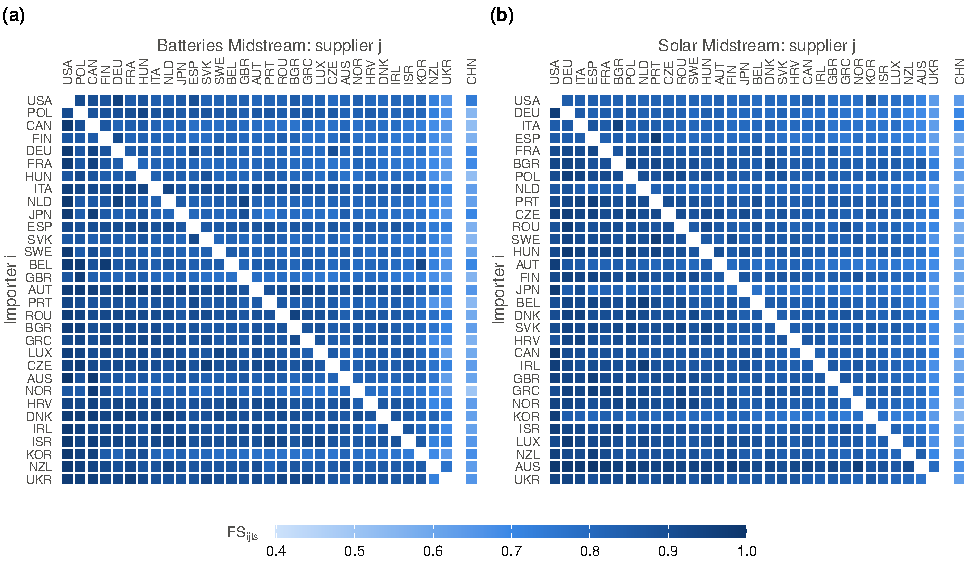
\includegraphics[width=\textwidth]{bilateral_fs_heatmap}
  \caption{Friendshore index among the core members, (a) Batteries Midstream and (b) Solar
  Midstream. Rows are importers $i$, columns suppliers $j$; colour is $\FS_{ijts}$
  (equation~\eqref{eq:fs_index}), the within-cell S-curve of the weighted mean of the components
  less the climate penalty. Rows and columns are the 31 core coalition members ordered by their mean
  rating as suppliers; the last column is China as a supplier to each core member. The diagonal is
  empty. Every dyad shown has an observed import component (importer's declaration or mirror).
  Source: \texttt{partner\_friendshore\_tbl.rds}.}
  \label{fig:bilateral_fs_heatmap}
\end{figure}

\paragraph{What makes a top supplier.} The leading suppliers of the United States (the United
Kingdom, Germany, Canada) and of Japan (the United States, Portugal, Austria) are all U.S.-leaning
except Thailand, seventh for Japan (Figure~\ref{fig:bilateral_fs_components}). Alignment is the largest
contribution to the top ten's composites (29.1 and 29.0 percent), followed by partner capability
(23.0 and 24.9), imports (18.7 and 20.1) and need (18.7 and 16.9); investment contributes 9.9 and 6.9
percent. China ranks 70th among the suppliers of the United States and 75th among those of Japan,
and would rank 10th and 8th without alignment. Because absent investment records drop out rather
than count as zero, and the summary keeps a dyad's five best cells, small aligned economies with a
few strong cells rank high: Estonia and Lithuania are the ninth and tenth suppliers of the United
States, and neither they nor the Netherlands, Ireland (both conduit centres, whose positions are
excluded) and Slovakia have an investment record in their five best cells. Scoring an absent record
at the lowest rank instead replaces all five in the United States' top ten, with Spain, Japan,
Poland, Korea and Belgium, but barely moves the headline index
(Section~\ref{subsec:robust_psi}).

\begin{figure}[tbp]
  \centering
  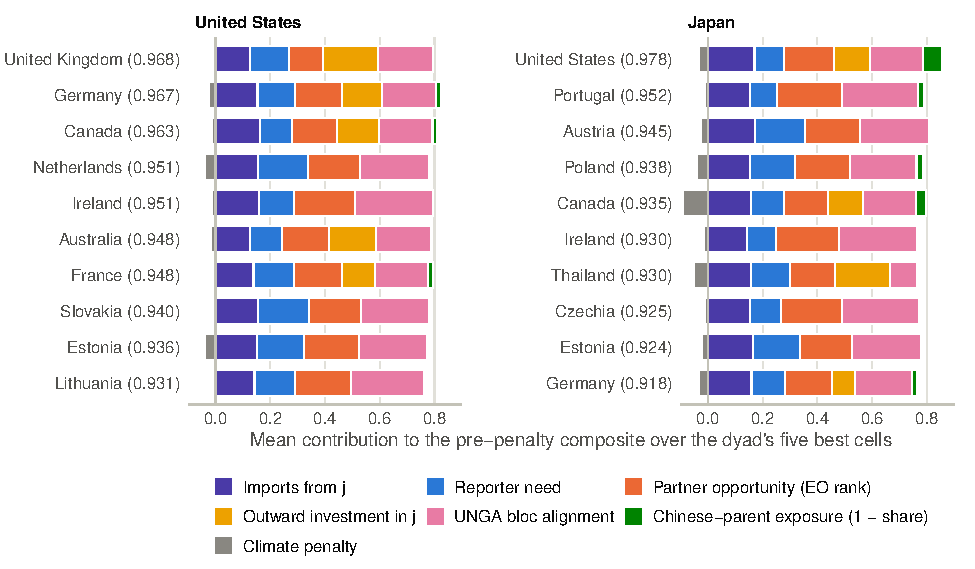
\includegraphics[width=\textwidth]{bilateral_fs_components}
  \caption{Composition of the Friendshore composite for the ten highest-ranked suppliers of the
  United States (left) and Japan (right). Each bar is the mean, over the five technology--stage
  cells behind the dyad's best-five summary $T^{\FS}_{ij}$ (in parentheses), of the weighted
  component contributions $w_c x_c/\sum_{c'\,\mathrm{obs}}w_{c'}$, which sum to the pre-penalty
  composite; the climate penalty is the negative segment. Components and weights: imports from $j$
  (2), reporter need (2), partner capability (2), outward investment in $j$ (2; IMF positions, or
  CM-FDI projects in Batteries, Electric Vehicles, Solar and Wind Midstream), UNGA bloc alignment
  (2) and Chinese-parent exposure scored as $1-$share (1, defined only in those four cells); the
  zero-weight reporter capability term is omitted. A missing segment means the component is
  unobserved for that dyad and dropped from the mean. Suppliers are ranked among partners that are
  sovereign and whose Friendshore dyad has an imputed weight share of at most 0.5 (158 for the
  United States, 170 for Japan). Source: \texttt{partner\_friendshore\_tbl.rds},
  \texttt{partner\_friendshore\_top5\_tbl.rds}; penalty recomputed from the technology emission
  index and the Climate Action Tracker ratings.}
  \label{fig:bilateral_fs_components}
\end{figure}

\paragraph{The alignment component.} Alignment carries weight 2 of 11 (18.2 percent) but 24.1
percent of the pre-penalty composite on average: for a core reporter it contributes 0.231 for a
U.S.-leaning partner, 0.115 for a nonaligned one and zero for a China-leaning one. Setting its weight
to zero changes the headline more than any other single choice examined: the Spearman correlation
with the headline $\PSI_j$ is 0.869 (0.716 for $C^{\FS}_j$), the median partner moves 17 places, and
China would rise from 44th to 3rd, India from 39th to 16th, Indonesia from 62nd to 15th and Russia
from 105th to 47th. The headline ranking is thus in large part a statement about political alignment
with the United States; a purely economic reading of supplier strength should use the variant
without it.

\paragraph{Chinese-parent exposure.} Of the 905 CM-FDI projects, 406 have a parent headquartered in
China, Hong Kong or Macao. The share is defined for 24 to 28 suppliers per covered cell, 47 economies
in all, 31 of them coalition members (Figure~\ref{fig:bilateral_cmfdi_exposure}); over the 94
supplier--technology cells outside China its median is 0.50, highest in solar (median 0.75) and
lowest in wind (0). Some partners on which the coalition relies are heavily exposed, among them
T\"urkiye, Thailand, Malaysia and Viet Nam, and in the core Korea (batteries 0.91) and Hungary
(electric vehicles 0.64). The component implements one channel, parent-company ownership, of the
common-mode upgrade proposed in the working paper on the Allied Industrial Base
\citep{neis2026allied}: plants in two supplier countries owned by
the same parent do not diversify a buyer's supply. With modest weight and narrow coverage its effect
on the headline is small (within-cell Spearman of $\FS$ with and without it 0.99; no $\PSI_j$ rank
moves by more than four places) but concentrated where it should be: the change in core members'
ratings correlates at $-0.93$ with the share, and China loses 0.085--0.095 per cell. The component
also raises the ratings of suppliers whose few foreign-invested plants have non-Chinese parents,
whoever those parents are: with it, the core's mean rating of Russia over its covered cell rises
from 0.32 to 0.40, and Argentina's from 0.42 to 0.50
(Figure~\ref{fig:bilateral_cmfdi_exposure}b). It measures the absence of Chinese ownership, not the
presence of trusted ownership. It sees
ownership of foreign-invested plants only, not dependence on Chinese equipment, precursors or
licences.

\begin{figure}[tbp]
  \centering
  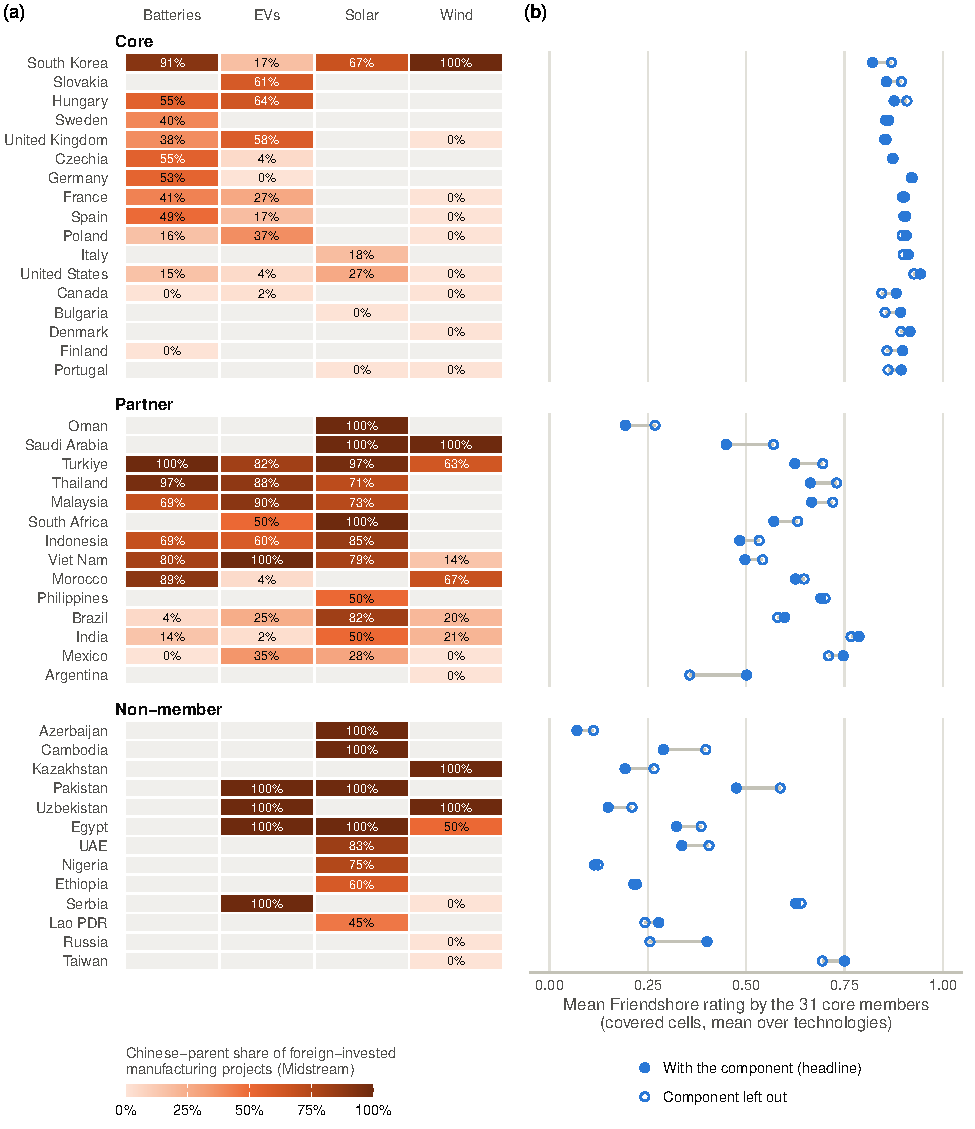
\includegraphics[width=0.93\textwidth]{bilateral_cmfdi_exposure}
  \caption{Chinese-parent ownership exposure of suppliers. Panel (a): for each economy hosting at
  least two foreign-invested manufacturing projects in a technology, the share of those projects
  owned by parents headquartered in China, Hong Kong or Macao (capital-weighted where capital is
  disclosed, by count otherwise; joint ventures attribute half to each parent), in the Midstream
  cells of batteries, electric vehicles, solar and wind; grey cells are undefined (fewer than two
  projects). Rows are grouped by coalition tier and ordered by the mean share; China, Hong Kong and
  Macao, set to one by construction, are omitted. Panel (b): the mean Friendshore rating of the
  economy by the 31 core members over its covered cells, with the component (filled) and with its
  weight set to zero and every later step re-run (open). Source: CM-FDI database, Net Zero
  Industrial Policy Lab, Johns Hopkins University (CC BY 4.0), 905 of 1,042 projects;
  \texttt{partner\_cm\_fdi\_exposure\_tbl.rds}, \texttt{partner\_friendshore\_tbl.rds}.}
  \label{fig:bilateral_cmfdi_exposure}
\end{figure}

\paragraph{The partner-level PSI.} In the headline view (Figure~\ref{fig:bilateral_psi_rank}) the
United States (0.936), Germany (0.934), the Netherlands, the United Kingdom, France, Italy, Spain,
Belgium, Poland and Czechia (0.904) rank highest. Core members hold 24 of the top 25 places (median
rank 16); the first non-member is Slovenia (25th), a member of the EU node. Partners rank lower
(median 64.5), from Saudi Arabia (38th) and India (39th) to Gabon (141st). China ranks 44th, a strong
market and a weak supplier in this view (21st on $C^{\PO}_j$, 57th on $C^{\FS}_j$), Taiwan 47th and
Switzerland 51st. Opportunity varies little across partners (standard deviation 0.031, against
0.190 for $C^{\FS}_j$ and $C^{\DP}_j$), so although nominally 40 percent of the index it accounts for
5.5 percent of the variance of $\PSI_j$ among the 130 partners with all three categories
(Friendshore 63.8, Development 30.7 percent).

\begin{figure}[tbp]
  \centering
  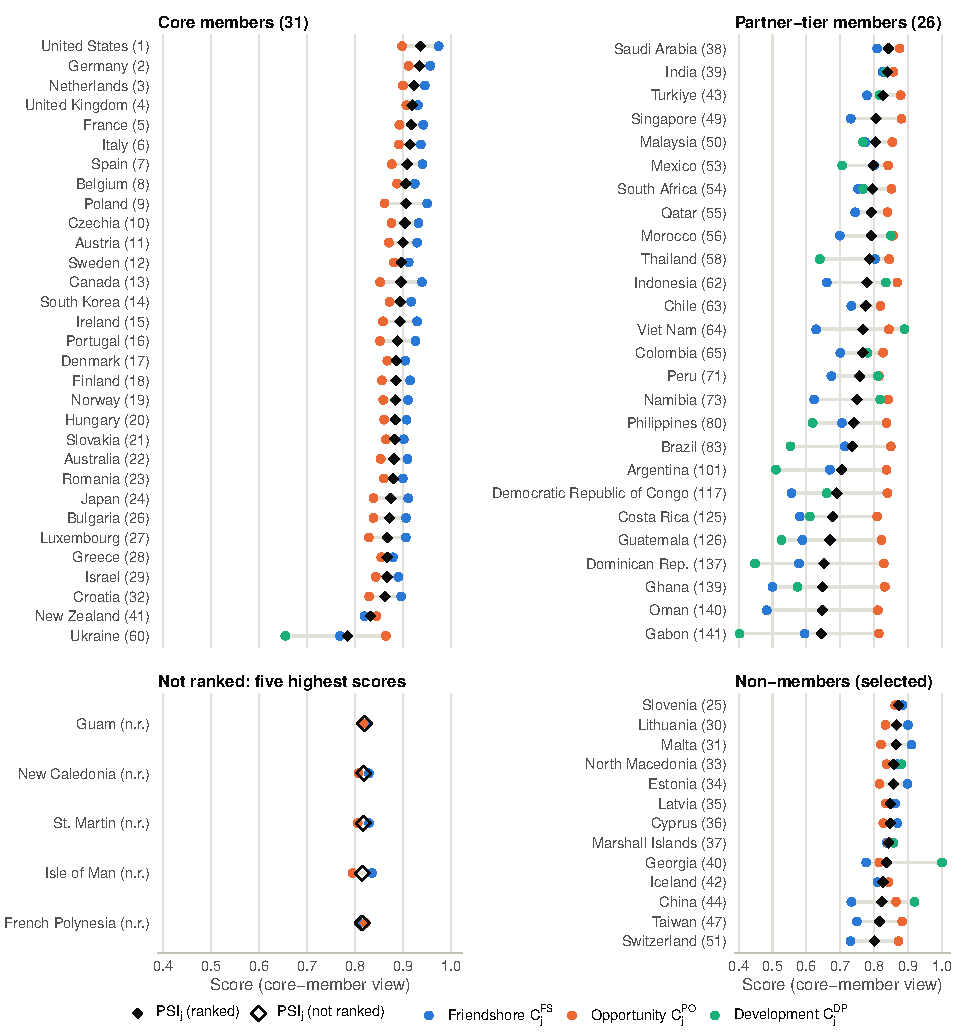
\includegraphics[width=\textwidth]{bilateral_psi_rank}
  \caption{Partnership Strength Index in the headline view. Diamonds are $\PSI_j$
  (equation~\eqref{eq:psi}) with $C^{\FS}_j$ and $C^{\PO}_j$ averaged over the 31 core coalition
  members as reporters; dots are the three category scores, Friendshore $C^{\FS}_j$, Partnership
  Opportunity $C^{\PO}_j$ and Development Potential $C^{\DP}_j$ (partners that are not high-income
  only). Panels: the 31 core members, the 26 partners, the ten highest-ranked non-members with
  China, Taiwan and Switzerland, and the five highest-scoring partners that are not ranked. Ranks
  in parentheses are among the 192 rankable partners (sovereign, imputed weight share at most 0.5);
  open diamonds and ``n.r.'' mark partners without a rank. Source: \texttt{psi\_tbl.rds}.}
  \label{fig:bilateral_psi_rank}
\end{figure}

\paragraph{Views of the index.} The core and full-coalition views agree closely (Spearman 0.981 over
192 ranked partners, median rank change 5, 13 of the top fifteen in common); the core and world views
(188 ranked) less so (0.881, median change 17, ten in common) (Table~\ref{tab:bilateral_psi_views}).
The views differ in how they place the large nonaligned and China-leaning economies: China is 44th,
9th and first in the core, full-coalition and world views, India 39th, 15th and 2nd, Indonesia 62nd,
32nd and 6th. The partners whose rating depends on who is asking are those whose alignment differs
from that of the core.

% Generated by scripts/paper/fig_bilateral.R; numbers in paper/results/bilateral.json (psi_views).
\begin{table}[t]
\centering
\begin{threeparttable}
\caption{The fifteen highest-ranked partners in the three views of the Partnership Strength Index}
\label{tab:bilateral_psi_views}
\footnotesize
\begin{tabular}{@{}r l S[table-format=1.3] l S[table-format=1.3] l S[table-format=1.3]@{}}
\toprule
 & \multicolumn{2}{c}{Core members (31 reporters)} & \multicolumn{2}{c}{Full coalition (57)} & \multicolumn{2}{c}{World (218)}\\
\cmidrule(lr){2-3}\cmidrule(lr){4-5}\cmidrule(l){6-7}
Rank & Partner & {$\PSI_j$} & Partner & {$\PSI_j$} & Partner & {$\PSI_j$}\\
\midrule
1 & United States & 0.936 & United States & 0.893 & China & 0.813\\
2 & Germany & 0.934 & Germany & 0.879 & India & 0.787\\
3 & Netherlands & 0.922 & France & 0.868 & France & 0.783\\
4 & United Kingdom & 0.919 & Netherlands & 0.864 & United States & 0.782\\
5 & France & 0.917 & Spain & 0.861 & Germany & 0.780\\
6 & Italy & 0.914 & United Kingdom & 0.857 & Indonesia & 0.768\\
7 & Spain & 0.908 & Italy & 0.854 & Netherlands & 0.764\\
8 & Belgium & 0.906 & South Korea & 0.852 & South Korea & 0.761\\
9 & Poland & 0.906 & China & 0.850 & Spain & 0.760\\
10 & Czechia & 0.904 & Belgium & 0.848 & United Kingdom & 0.757\\
11 & Austria & 0.900 & Canada & 0.847 & Italy & 0.755\\
12 & Sweden & 0.896 & Poland & 0.840 & Viet Nam & 0.753\\
13 & Canada & 0.896 & Czechia & 0.838 & Canada & 0.750\\
14 & South Korea & 0.894 & Austria & 0.838 & Austria & 0.746\\
15 & Ireland & 0.893 & India & 0.836 & Malaysia & 0.746\\
\bottomrule
\end{tabular}
\begin{tablenotes}[flushleft]\footnotesize
\item \textit{Notes:} $\PSI_j$ (equation~\eqref{eq:psi}) with $C^{\FS}_j$ and $C^{\PO}_j$ averaged over the reporters of each view: the 31 core coalition members (the headline), the 57 core and partner-tier members, and every other reporter (218 per partner). Ranks among the rankable partners of each view (sovereign, imputed weight share at most 0.5): 192, 192 and 188 partners. Spearman correlations of $\PSI_j$ across the partners ranked in both views: core and full coalition 0.981 (192), core and world 0.881 (188), full coalition and world 0.948 (188). Source: \texttt{psi\_tbl.rds}, \texttt{psi\_full\_coalition\_tbl.rds}, \texttt{psi\_world\_tbl.rds}; \texttt{scripts/paper/fig\_bilateral.R}.
\end{tablenotes}
\end{threeparttable}
\end{table}


\paragraph{Supplier and market views of the same edge.} For coalition pairs, the importer's
Friendshore rating of a supplier and the supplier's Opportunity rating of that importer as a market
agree to a degree (Figure~\ref{fig:bilateral_fs_po}; Spearman 0.715 over 95,312 matched cells),
partly through the shared capability term. Alignment, which enters only Friendshore, separates them:
Friendshore exceeds Opportunity by 0.157 on average for same-bloc pairs and falls short by 0.24 for
opposite blocs. The highest dyadic $\PSI_{ij}$ is Canada's rating of the United States (0.981).

\begin{figure}[tbp]
  \centering
  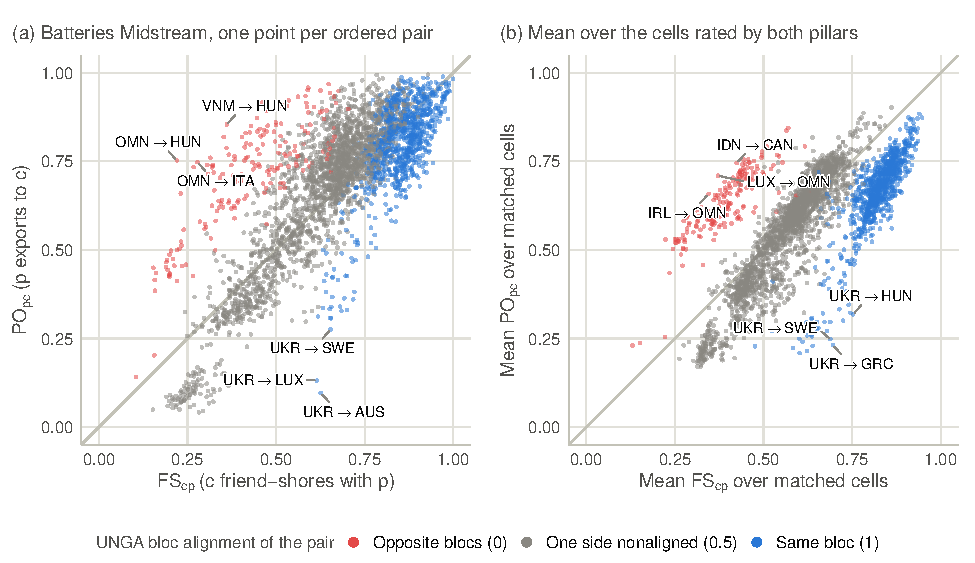
\includegraphics[width=\textwidth]{bilateral_fs_po}
  \caption{Supplier and market ratings of the same supply edge, coalition members. Horizontal:
  $\FS_{cp}$, member $c$'s Friendshore rating of member $p$ as a supplier; vertical: $\PO_{pc}$,
  $p$'s Opportunity rating of $c$ as a market. Panel (a): Batteries Midstream, one point per ordered
  pair of the 57 members (3,192 pairs). Panel (b): mean over the technology--stage cells rated by
  both pillars (28 to 30 per pair). Colour is the pair's dyadic UNGA alignment (1 same bloc, 0.5 when
  either is nonaligned, 0 opposite blocs); the line is the diagonal; the three pairs most favoured by
  each view are labelled. Source: \texttt{partner\_friendshore\_tbl.rds},
  \texttt{partner\_opportunity\_tbl.rds}.}
  \label{fig:bilateral_fs_po}
\end{figure}

\paragraph{Development potential.} Among the 125 ranked partners, Georgia, Mongolia and Mauritius
(1.00), Tuvalu and China (0.919) have the highest best-five summaries; the aid components, 35
percent of the nominal weight, provide 43.7 percent of the composite in their best cells. China's
score is a reminder that the pillar rates absorptive capacity, not alignment.
